\chapter{Design}
META

\section{Components}

We split the project into a number of components based on the requirements, \unsure{ change to this: different iterations of prototypes will be used to test these components?} these components are implemented in different prototype iterations, and thereby tested. 



The features that are planned for the product (using the requirements), are split into components. 

The idea is that the components are mostly separate from each other and each deal with different functionality and concerns. 

Each component is intended to be a complete piece of functionality.

Note that this is not a class diagram over the system architecture that we are going to implement, this follows in section \todo{add ref to class diagram ref{}}. Instead, this component diagram describes only a separation of concerns and dependencies.





\begin{figure}[h]
    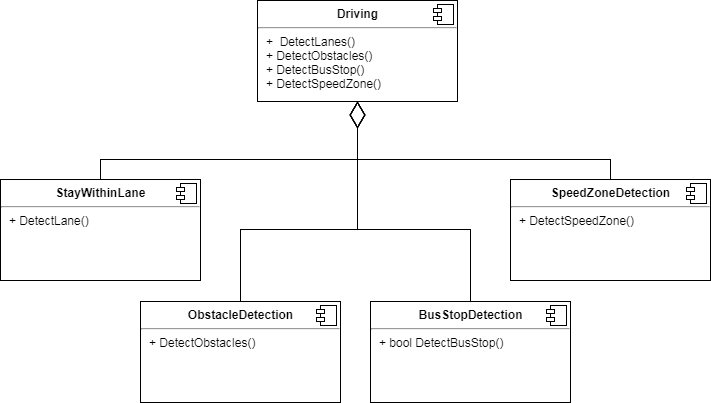
\includegraphics[width=\textwidth]{Images/Design/componentDiagram.png}
    \caption{Major components of functionality in the program}
\end{figure}
EXPLAIN ANYTHING THATS STILL UNCLEAR

%Jeg er ikke overbevist om at ovenstående diagram er vildt vigtigt når vi nu alligevel har det nedenstående

\section{Software Architecture}

Diagram over our planned implementation, showing both classes and interfaces
Add function calls to the arrows? Or rather functions to the classes themselves?
This is still not one-to-one with implementation. The API's don't communicate directly with their corresponding sensors, instead they all query the NXT block, which gives access to different functions dependant on which sensors are connected.
Mention external bluetooth-sender program

\begin{figure}[h]
    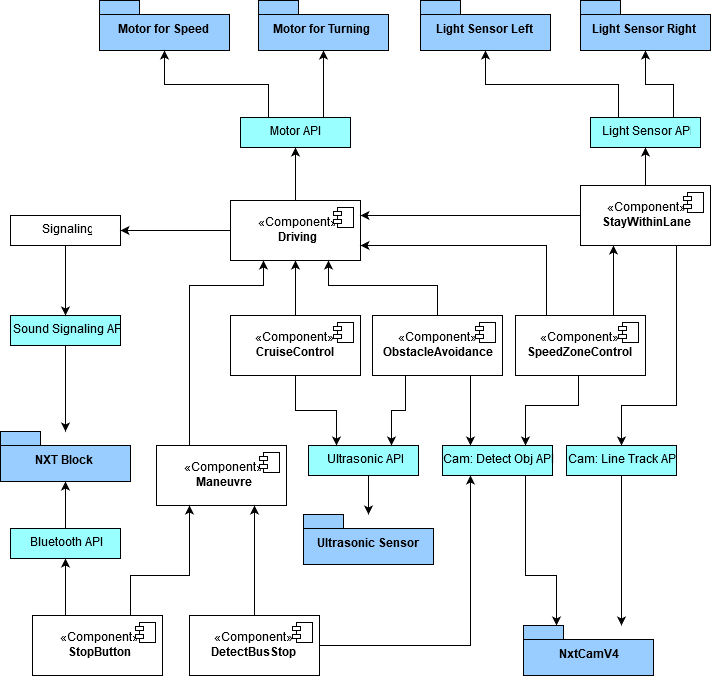
\includegraphics[width=\textwidth]{Images/Design/architectureClassDiagram.png}
    \caption{Diagram of the program architecture and how these communicate with each other}
\end{figure}

These classes will be used for implementing the program! It is still, however, kind of an abstraction.
In truth, the API's don't communicate directly with their corresponding sensors and actuators (and nxt block). 
Instead, they include libraries that facilitate this communication. 
The figure above shows the implementation of our model, ie. the software of the bus that we write ourselves.

Above this, there are many layers of abstraction in this project before one actually reaches the hardware level of the sensors. These are explained in the following section. 

\section{System Architecture}

Abstraction Layers, OS and nxtOSEK, lejOS?, ref to nxtOSEK section?

ABSTRACTION LAYER DIAGRAM
The frame "Components" in the figure are the components planned in the Software Architecture section. 

The diagram showing layers of abstraction in our design, including our NXTosek operating system

inclue ecrobot\_interface.h in source code
Write about the OSEK standard
And thereby also OIL



%\chapter{Design}
\section{Design of the track} \todo{This section needs to be checked for correctness.}

In order to fulfil the requirements of the project a track for the bus will have to be made, but before we can create the track it will first have to be designed.

The track should have two lanes, to mimic the pre-existing infrastructure with bidirectional roads. The track should furthermore have bus stops that the vehicle can drive into, such that passengers can get on/off the bus.
Furthermore the track should be designed to the scale of the bus, such that the turning rate of a corner should fit the maximum turning radius of the bus, and the width of the road should be designed after real danish roads based on the laws given by the danish road directorate \ref{} \todo{[MANLGER KILDE]}. Therefore the track needs be designed such that the bus has the needed space to turn around the corners without needing to reverse.

To help the sensors detect when to switch to a bus stop lane, the track should have special formed/coloured objects placed next to the bus stops, which the sensor(s) can recognise. Furthermore if any people are standing at the bus stop to get onto the bus, they should be placed close to the bus stop sign.

To draw the track that the bus will drive on, black tape should be used such that the sensors that perform line tracking can more easily detect and stay within the lines. Black has been chosen over white, even though white is normally used to draw track lines. But since white can be hard to detect because of light reflection the tracks will use black lines, this is to focus on a more complete bus implementation rather than focusing on tracking the lanes themselves.
\input{Documents/3Design/Design/Design_of_car}